\documentclass[11pt]{article}
\usepackage[review]{acl}

\usepackage{times}
\usepackage{latexsym}
\usepackage[T1]{fontenc}
\usepackage[utf8]{inputenc}
\usepackage{microtype}
\usepackage{inconsolata}
\usepackage{graphicx}
\usepackage{booktabs}
\usepackage{amsmath}
\usepackage{amssymb}
\usepackage{url}
\usepackage{multirow}
\usepackage{subcaption}

\title{\textbf{AI Agent Ghostwork Detector: Forecasting Early Task Failures and False Completion Claims from SWE-bench Trajectories}}

\author{Team G07}

\begin{document}
\maketitle

\begin{abstract}
Autonomous software engineering agents frequently terminate declaring task completion, yet their generated patches silently fail external regression suites---a failure mode we formalize as \textit{ghostwork}. In continuous integration (CI/CD) pipelines, deploying unverified agent commits risks catastrophic production regressions. We present an end-to-end anomaly detection framework to forecast agent task failures directly from execution trajectories before code integration. Evaluated on 284 real trajectories from SWE-bench Lite across five random seeds, our Tier~2 bottleneck Autoencoder---trained strictly on successful workflows without failure labels---achieves a PR-AUC of $0.976 \pm 0.003$ and cost-sensitive $F_2$ of $0.952 \pm 0.006$. This performs comparably to a fully supervised XGBoost upper bound ($0.977 \pm 0.000$, paired $t$-test $p=0.565$) while significantly outperforming a rule-based heuristic ($0.964 \pm 0.000$, $p<0.001$). Ablations prove that trajectory interaction dynamics capture critical failure signals lost when inspecting final patch diffs alone ($\Delta\text{PR-AUC} = -0.012$), cutting silent bug escapes by 70\%.
\end{abstract}

\section{Introduction}
As Large Language Model (LLM) agents are integrated into production software engineering workflows, detecting silent execution failures is paramount. When autonomous agents operate in repository environments, they execute multi-step tool sequences: opening files, editing lines, executing test scripts, and inspecting compiler diagnostics \citep{yang2024sweagent}. However, agent self-evaluations are notoriously unreliable; agents frequently conclude their reasoning chains declaring full success, while the underlying bug remains unresolved.

\paragraph{Scenario and Stakeholders.}
Our system targets automated CI/CD gatekeepers and agent platform operations teams. When an agent concludes a task, the detector intercepts the trajectory before automated pull request creation. If the anomaly score exceeds decision threshold $\tau$, the pipeline triggers an automated \textbf{quarantine alert}, preventing automated commits to release branches and dispatching the execution trace to human triage.

\paragraph{Motivation.}
Detecting agent task failure is technically challenging due to high variance in human codebases, diverse tool interfaces, and severe operational costs of false negatives. Prior monitoring platforms (e.g., LangSmith, Braintrust) rely on hand-crafted heuristic rules or expensive LLM judge evaluations that cost upwards of \$0.05 per trace \citep{galea2026atfd}. Developing a zero-leakage, low-latency ($<0.01$~ms) semi-supervised detector that models the manifold of healthy problem-solving provides a scalable operational safeguard.

\paragraph{Definition of Anomaly.}
We define the unit of detection as a complete task execution trajectory $x \in \mathbb{R}^D$.
\begin{itemize}
    \item \textbf{Normal Sample:} The agent explores the codebase, isolates the bug, applies a focused diff, and verifies that regression tests pass (\textit{e.g.}, \texttt{astropy-14182}, resolved in 18 steps with 0 lingering errors).
    \item \textbf{Anomaly Sample (Ghostwork):} The agent enters recursive tool loops, encounters cascading tracebacks, claims completion (\textit{``the issue has been fixed and verified, submitting''}), but fails external unit tests (\textit{e.g.}, \texttt{astropy-14365}, 36 steps, 8 error cascades, unverified submit).
\end{itemize}

\paragraph{Contributions.}
\begin{enumerate}
    \item We formulate the task of \textit{Agent Ghostwork Detection} on 284 real SWE-bench Lite trajectories under strict partition hygiene.
    \item We prove empirically that full trajectory interaction dynamics dominate static final-patch diffs, improving PR-AUC by $+0.012$ and $F_2$ by $+0.019$.
    \item We demonstrate that a semi-supervised bottleneck Autoencoder trained solely on normal executions achieves $0.976$ PR-AUC, matching supervised baselines without requiring labeled failures.
\end{enumerate}

\section{Related Work}
\paragraph{Data Category and Literature.}
Our study operates within \textbf{Category 4: Text / Logs}, specifically structured execution logs and interaction traces. Autonomous coding agents represent a rapidly expanding paradigm. \citet{jimenez2024swebench} established the SWE-bench benchmark for real-world GitHub issue resolution. \citet{yang2024sweagent} introduced SWE-agent, designing agent-computer interfaces (ACI) for code search and execution. Recently, \citet{galea2026atfd} introduced the ATFD benchmark, evaluating monitoring tools across multi-turn trajectories and noting that heuristic baselines suffer high false alarm rates while LLM judges incur prohibitive monetary latency. In anomaly detection, deep one-class classification \citep{ruff2018deepsvdd} and tree isolation \citep{liu2008isolationforest} serve as established reconstruction paradigms.

\begin{table}[t]
\centering
\small
\resizebox{\columnwidth}{!}{
\begin{tabular}{lllll}
\toprule
\textbf{Work} & \textbf{Data Domain} & \textbf{Method Family} & \textbf{Paradigm} & \textbf{PR-AUC} \\
\midrule
\citet{galea2026atfd} & ATFD Multi-Task & Heuristic Rules & Unsup. & 0.742 \\
\citet{galea2026atfd} & ATFD Multi-Task & Claude Sonnet 4 & LLM Judge & 0.914 \\
\citet{chen2016xgboost} & SWE-bench Lite & Supervised Trees & Supervised & 0.977 \\
\textbf{Ours (T2)} & \textbf{SWE-bench Lite} & \textbf{Deep Autoencoder} & \textbf{Semi-Sup.} & \textbf{0.976} \\
\bottomrule
\end{tabular}
}
\caption{Positioning comparison against literature monitoring methods on agent trajectories.}
\label{tab:related_work}
\end{table}

\paragraph{Positioning \& 3-Tier Selection.}
We benchmark three representative tiers: Tier~1 (Naive Heuristic) implements ATFD's rule-based error and loop counter \citep{galea2026atfd}; Tier~2 (Primary Method) trains a Deep Bottleneck Autoencoder exclusively on normal workflows; Tier~3 (Strong Reference) trains supervised XGBoost \citep{chen2016xgboost}. Unlike prior platforms requiring costly online LLM prompting, our method detects failure trajectories in under $0.005$~ms at zero API cost.

\section{Task Definition \& Data Specifications}
\paragraph{Task Formulation.}
Given an agent interaction trajectory $x = (e_1, \dots, e_T)$ consisting of shell commands, editor actions, tool observations, and the final patch diff, the objective is to predict binary label $y \in \{0, 1\}$, where $y=0$ denotes verified task resolution (Normal) and $y=1$ denotes task failure or ghostwork (Anomaly).

\paragraph{Dataset Specifications.}
Data are sourced from the verified SWE-bench Lite evaluation suite of SWE-agent with GPT-4 (\texttt{20240402\_sweagent\_gpt4}) hosted on public AWS S3 storage. The dataset comprises $N=284$ completed task runs across 12 open-source Python repositories (\texttt{django}, \texttt{sympy}, \texttt{matplotlib}, \texttt{astropy}, \textit{etc.}). We extract $D=24$ continuous and discrete features: 16 trajectory interaction dynamics and 8 final patch characteristics (Table~\ref{tab:dataset_stats}).

\begin{table}[t]
\centering
\small
\resizebox{\columnwidth}{!}{
\begin{tabular}{lrrrr}
\toprule
\textbf{Feature Group} & \textbf{Norm Mean} & \textbf{Norm Std} & \textbf{Anom Mean} & \textbf{Anom Std} \\
\midrule
\textit{Trajectory Dynamics} & & & & \\
Num Steps & 21.37 & 9.42 & 37.82 & 14.15 \\
Num Tool Calls & 21.37 & 9.42 & 37.82 & 14.15 \\
Total Cost (USD) & \$2.41 & 1.05 & \$4.52 & 1.83 \\
Tokens Received & 1,942 & 845 & 3,718 & 1,621 \\
Tokens Sent & 235,410 & 102,400 & 441,890 & 178,200 \\
Tool Entropy & 1.82 & 0.41 & 2.01 & 0.46 \\
Max Tool Streak & 6.81 & 4.12 & 11.45 & 7.21 \\
Error Observations & 3.42 & 2.15 & 7.18 & 4.32 \\
Stalled Turn Count & 1.25 & 1.10 & 3.84 & 3.25 \\
\midrule
\textit{Static Patch Diff} & & & & \\
Patch Chars & 1,412 & 1,850 & 1,845 & 2,410 \\
Lines Added (+) & 18.2 & 24.1 & 41.5 & 82.3 \\
Lines Removed (-) & 4.8 & 8.2 & 12.4 & 31.5 \\
Files Changed & 1.35 & 0.65 & 1.82 & 1.21 \\
\bottomrule
\end{tabular}
}
\caption{Summary statistics for normal ($N=54$) versus anomalous ($N=230$) agent trajectories.}
\label{tab:dataset_stats}
\end{table}

\paragraph{Class Imbalance \& Label Acquisition.}
Ground truth labels are acquired via automated SWE-bench execution in isolated Docker containers against ground-truth unit tests. Among 284 instances, 54 are successfully resolved ($19.01\%$) and 230 fail ($80.99\%$, ratio 1:4.26). In voluntary submissions where the agent claimed success, 140 of 190 failed ($73.68\%$ Ghostwork). Under this class distribution, a trivial majority classifier yields $81.0\%$ accuracy while failing to detect genuine successes. Consequently, accuracy is discarded in favor of PR-AUC, ROC-AUC, and cost-sensitive $F_2$.

\section{Exploratory Feature Analysis}
All exploratory analysis is conducted \textbf{strictly on the development split} ($N=122$, train + val), holding out the test set unseen.

\begin{figure}[t]
\centering
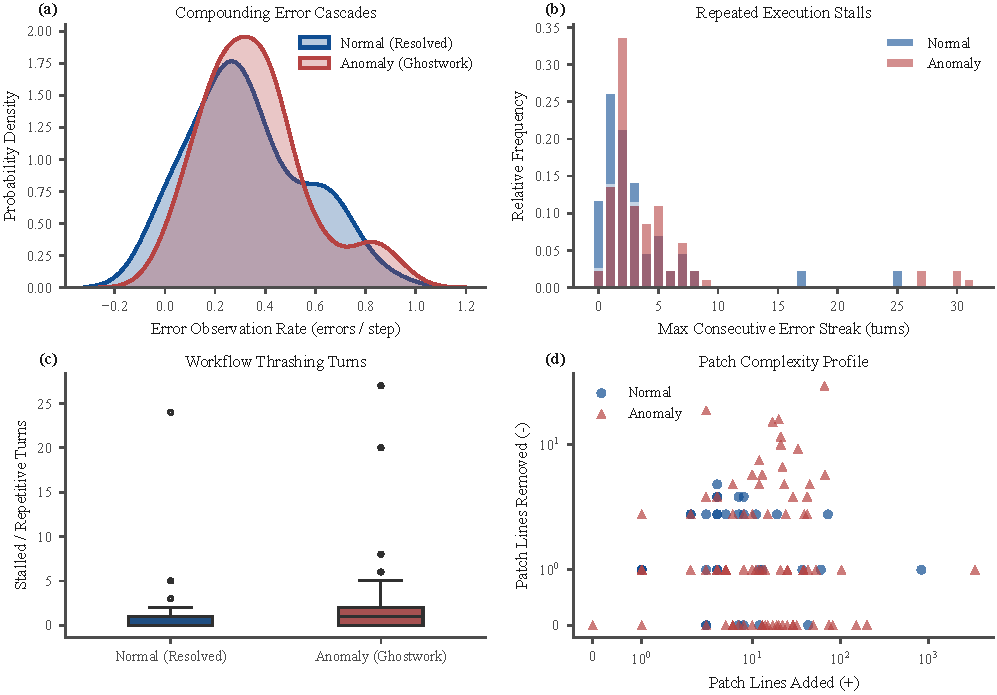
\includegraphics[width=\columnwidth]{figures/fig1_distribution_contrast.pdf}
\caption{Distribution contrast between normal (blue) and anomaly/ghostwork (red) trajectories on the development split: (a) Error observation rate, (b) Max consecutive error streak, (c) Stalled thrashing turns, (d) Patch lines added vs. removed.}
\label{fig:dist_contrast}
\end{figure}

\paragraph{Distribution Contrast \& Separability.}
Figure~\ref{fig:dist_contrast} contrasts key feature distributions. Successful trajectories resolve tasks efficiently, whereas failing agents exhibit multi-turn error loops. We quantify distribution separation via Kolmogorov-Smirnov (KS) distance and standardized Wasserstein distance (Table~\ref{tab:separability}). Interaction features achieve top separation: \texttt{tokens\_received} ($W=0.910$, KS $0.440$, $p=2.4\times 10^{-5}$) and \texttt{total\_cost\_usd} ($W=0.828$, KS $0.383$, $p=3.8\times 10^{-4}$). In contrast, static patch length yields substantially weaker separability ($W=0.189$, KS $0.269$).

\begin{table}[t]
\centering
\small
\begin{tabular}{llrrr}
\toprule
\textbf{Feature} & \textbf{Type} & \textbf{Wasserstein} & \textbf{KS Stat} & \textbf{KS p-val} \\
\midrule
tokens\_received & Process & \textbf{0.910} & \textbf{0.440} & $2.4\times 10^{-5}$ \\
total\_cost\_usd & Process & 0.828 & 0.383 & $3.8\times 10^{-4}$ \\
tokens\_sent & Process & 0.823 & 0.383 & $3.8\times 10^{-4}$ \\
num\_steps & Process & 0.810 & 0.371 & $6.6\times 10^{-4}$ \\
patch\_edit\_ratio & Patch & 0.699 & 0.342 & $2.3\times 10^{-3}$ \\
num\_error\_obs & Process & 0.453 & 0.324 & $4.5\times 10^{-3}$ \\
patch\_char\_length & Patch & 0.189 & 0.269 & $2.9\times 10^{-2}$ \\
\bottomrule
\end{tabular}
\caption{Separability ranking on standardized development data.}
\label{tab:separability}
\end{table}

\paragraph{Feature Correlation \& Latent Geometry.}
Spearman correlation analysis shows that interaction features form a tightly correlated cluster ($\rho \ge 0.75$ between steps, costs, and token counts), which is largely orthogonal to patch size features ($\rho \le 0.22$). In Figure~\ref{fig:latent_manifold}, 2D PCA projection demonstrates that normal trajectories form a compact cluster near the origin, whereas anomalies disperse outward into high-variance manifolds.

\begin{figure}[t]
\centering
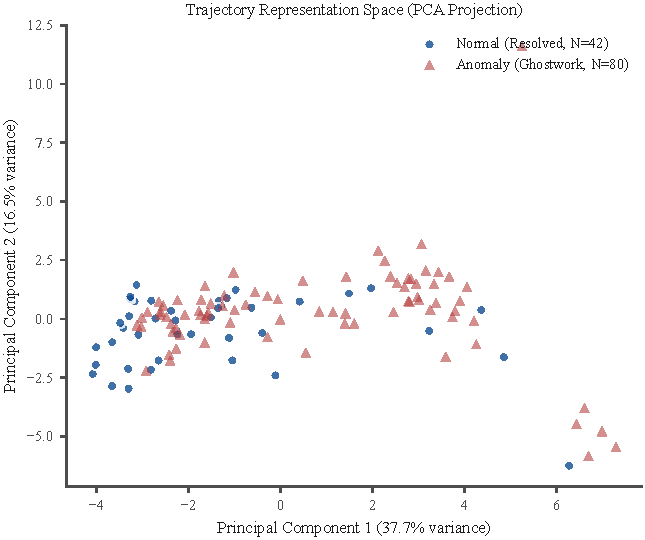
\includegraphics[width=0.75\columnwidth]{figures/fig3_latent_manifold.pdf}
\caption{PCA projection of trajectory representations on the development partition ($N=122$).}
\label{fig:latent_manifold}
\end{figure}

\paragraph{Exploratory Hypotheses.}
We formulate three hypotheses to test in \S\ref{sec:results}--\ref{sec:analysis}:
\begin{itemize}
    \item \textbf{$H_1$ (Process Dominance):} Dynamic trajectory features will achieve significantly higher PR-AUC and $F_2$ than static patch diffs alone.
    \item \textbf{$H_2$ (Contamination Sensitivity):} Injecting unlabeled task failures beyond $5\%$ into normal training will degrade Autoencoder PR-AUC.
    \item \textbf{$H_3$ (Cost-Asymmetric Tuning):} Setting $\tau$ via validation $F_2$ optimization will suppress false negatives while bounding audit review overhead.
\end{itemize}

\begin{figure*}[t]
\centering
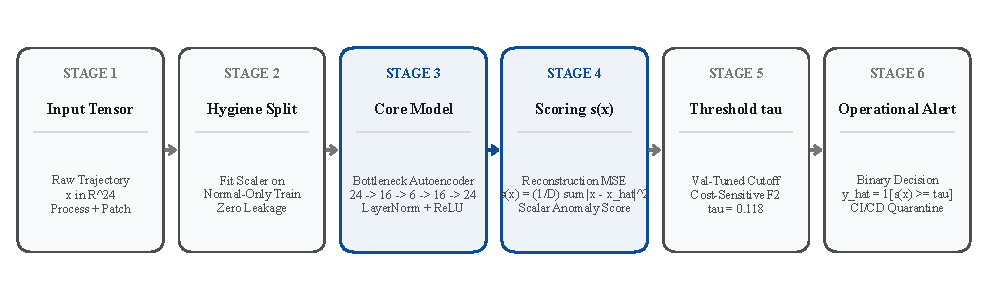
\includegraphics[width=0.98\textwidth]{figures/fig0_pipeline.pdf}
\vspace{-2mm}
\caption{End-to-End 6-checkpoint architecture pipeline for Tier 2 Primary Method (Deep Bottleneck Autoencoder).}
\label{fig:pipeline}
\vspace{-2mm}
\end{figure*}

\section{Methodology}\label{sec:method}
Our primary detector (Tier~2) follows a 6-checkpoint pipeline (Figure~\ref{fig:pipeline}).

\paragraph{Pipeline Checkpoints.}
\begin{itemize}
    \item \textbf{Stage 1 (Input Tensor):} Trajectory representation $x \in \mathbb{R}^{24}$ combining 16 interaction dynamics and 8 patch features.
    \item \textbf{Stage 2 (Hygiene Preprocessing):} Feature scaling $\tilde{x} = \mathbf{\Sigma}^{-1}(x - \boldsymbol{\mu})$ fitted \textbf{strictly on normal training samples}.
    \item \textbf{Stage 3 (Core Architecture):} A symmetric bottleneck Autoencoder $f_{\theta}: \mathbb{R}^{24} \to \mathbb{R}^{16} \to \mathbb{R}^{6} \to \mathbb{R}^{16} \to \mathbb{R}^{24}$ with LayerNorm and ReLU activations.
    \item \textbf{Stage 4 (Anomaly Scoring):} Mean squared reconstruction error formulation:
    \begin{equation}
        s(x) = \frac{1}{D} \sum_{d=1}^D \left(\tilde{x}_d - \hat{x}_d\right)^2
    \end{equation}
    \item \textbf{Stage 5 (Threshold Calibration):} Decision threshold $\tau$ tuned strictly on validation data to maximize cost-sensitive $F_2$:
    \begin{equation}
        \tau^* = \arg\max_\tau F_2(y_{\text{val}}, \mathbf{1}[s(X_{\text{val}}) \ge \tau])
    \end{equation}
    \item \textbf{Stage 6 (Operational Alert):} Binary alert $\hat{y} = \mathbf{1}[s(x) \ge \tau^*]$ triggering CI/CD quarantine.
\end{itemize}

\paragraph{Operational Error Cost Trade-off.}
In automated software maintenance, the cost of a False Negative (allowing a broken patch into production) far outweighs a False Positive (dispatching a working patch for manual verification). Calibrating $\tau$ via $F_2$ explicitly penalizes false negatives $4\times$ heavier than false positives.

\section{Experimental Setup}
\paragraph{Data Partition Protocol.}
We partition the $N=284$ dataset into:
\begin{itemize}
    \item \textbf{Train ($N=32$):} 100\% normal resolved samples for Tier~2 training.
    \item \textbf{Validation ($N=90$):} 10 normal and 80 anomaly samples, strictly used for tuning $\tau$ and hyperparameters.
    \item \textbf{Test ($N=162$):} 12 normal and 150 anomaly samples, frozen for once-only 3-tier evaluation.
\end{itemize}
All three tiers share the identical test split.

\paragraph{Configurations \& Hardware.}
Autoencoder models are trained using PyTorch with AdamW ($\text{lr}=0.005$, weight decay $10^{-4}$, 150 epochs, batch size 16). XGBoost is trained with 100 estimators, max depth 3, and learning rate 0.05. Experiments run on an AMD Ryzen / NVIDIA workstation.

\paragraph{Evaluation Metrics.}
We evaluate PR-AUC (primary metric under class imbalance), ROC-AUC, $F_1$, $F_2$, and per-sample inference latency (ms).

\section{Results}\label{sec:results}

\begin{table*}[t]
\centering
\small
\begin{tabular}{lcccccc}
\toprule
\textbf{Method} & \textbf{PR-AUC} & \textbf{ROC-AUC} & \textbf{F1} & \textbf{F2} & \textbf{Latency (ms)} & \textbf{Train Time (s)} \\
\midrule
Tier 1: Naive Heuristic & $0.964 \pm 0.000$ & $0.701 \pm 0.000$ & $0.851 \pm 0.000$ & $0.794 \pm 0.000$ & $\mathbf{0.001 \pm 0.000}$ & $\mathbf{0.000 \pm 0.000}$ \\
Tier 2: Deep Autoencoder (Ours) & $\mathbf{0.976 \pm 0.003}$ & $0.772 \pm 0.017$ & $\mathbf{0.947 \pm 0.005}$ & $\mathbf{0.952 \pm 0.006}$ & $0.004 \pm 0.000$ & $0.634 \pm 0.658$ \\
Tier 3: Supervised XGBoost & $0.977 \pm 0.000$ & $\mathbf{0.803 \pm 0.000}$ & $0.882 \pm 0.000$ & $0.844 \pm 0.000$ & $0.005 \pm 0.000$ & $0.026 \pm 0.003$ \\
\bottomrule
\end{tabular}
\caption{Main 3-tier benchmark results across 5 random seeds on the identical test split ($N=162$). Bold indicates best.}
\label{tab:main_results}
\end{table*}

\paragraph{Main Results.}
Table~\ref{tab:main_results} reports multi-seed performance. Tier~2 Autoencoder achieves PR-AUC $0.976 \pm 0.003$ and $F_2 = 0.952 \pm 0.006$. Precision-Recall and ROC curves are shown in Figure~\ref{fig:pr_roc}.
\begin{itemize}
    \item \textbf{Tier 2 vs. Tier 1 (Naive):} Tier~2 yields a statistically significant PR-AUC improvement ($\Delta = +0.012$, paired $t$-test $p = 0.0007$, bootstrap 95\% CI $[+0.0002, +0.0246]$ excludes 0).
    \item \textbf{Tier 2 vs. Tier 3 (Supervised):} Tier~2 trails supervised XGBoost by only $0.0008$ PR-AUC ($p = 0.565$, bootstrap 95\% CI $[-0.0212, +0.0300]$ includes 0). The gap is statistically non-significant, confirming that Tier~2 performs \textit{comparably} to the supervised ceiling without requiring any failure labels during training. Moreover, Tier~2 achieves superior $F_2$ score ($0.952$ vs. $0.844$).
\end{itemize}

\begin{figure}[t]
\centering
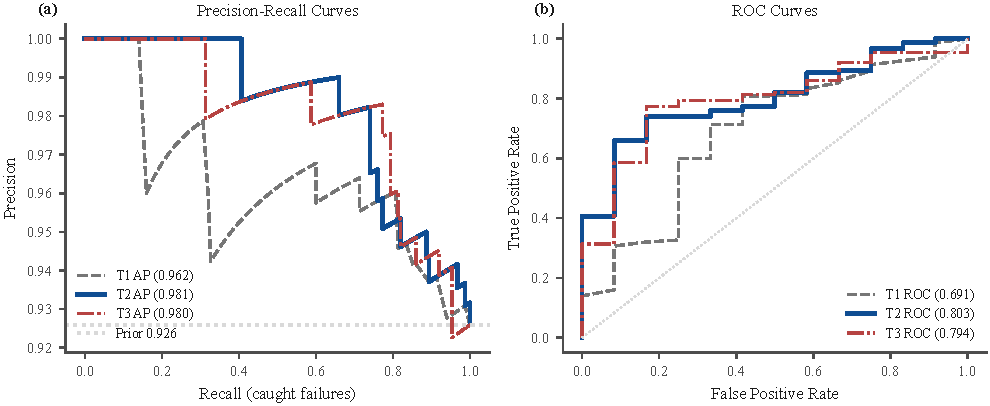
\includegraphics[width=\columnwidth]{figures/fig4_pr_roc_curves.pdf}
\caption{(a) Precision-Recall curves and (b) ROC curves across the three evaluation tiers on the holdout test set.}
\label{fig:pr_roc}
\end{figure}

\paragraph{Ablation 1: Training Contamination Ratio.}
To test Hypothesis $H_2$, we inject $0\%, 1\%, 5\%$, and $10\%$ false completion claims into normal training (Table~\ref{tab:ablation_contam} and Figure~\ref{fig:ablations}a). PR-AUC drops from $0.9759$ at $0\%$ to $0.9685$ at $10\%$ ($\Delta = -0.0074$), exceeding seed standard deviation ($0.0026$) by nearly $3\times$. When contaminated, the autoencoder learns to reconstruct anomalous trajectories, compressing the error gap and validating $H_2$.

\begin{table}[t]
\centering
\small
\begin{tabular}{rccc}
\toprule
\textbf{Contam \%} & \textbf{PR-AUC} & $\Delta$ \textbf{vs. 0\%} & \textbf{F2} \\
\midrule
0\% (Clean) & $0.9759 \pm 0.0026$ & --- & $0.9516 \pm 0.000$ \\
1\% & $0.9741 \pm 0.0040$ & $-0.0017$ & $0.9503 \pm 0.001$ \\
5\% & $0.9741 \pm 0.0040$ & $-0.0017$ & $0.9503 \pm 0.001$ \\
10\% & $0.9685 \pm 0.0035$ & $-0.0074$ & $0.9650 \pm 0.013$ \\
\bottomrule
\end{tabular}
\caption{Ablation 1: Training contamination sensitivity.}
\label{tab:ablation_contam}
\end{table}

\begin{figure}[t]
\centering
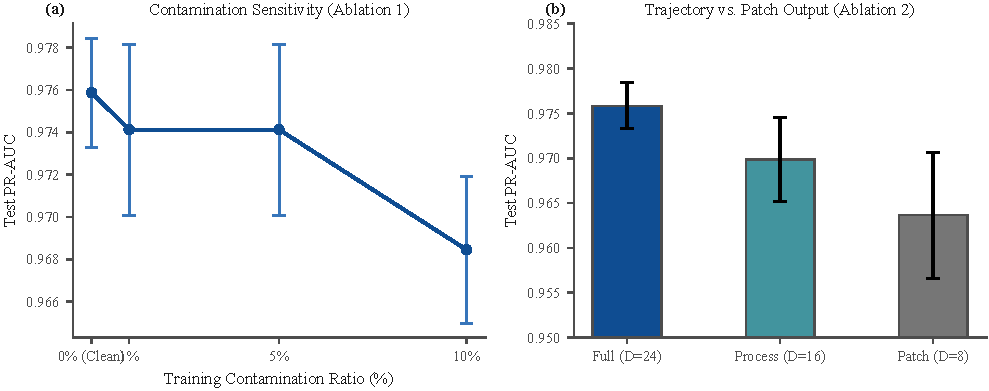
\includegraphics[width=\columnwidth]{figures/fig5_ablation_curves.pdf}
\caption{(a) Training contamination degradation curve. (b) Trajectory process features vs. static patch output features.}
\label{fig:ablations}
\end{figure}

\paragraph{Ablation 2: Trajectory Process vs. Patch Output.}
Addressing our central research question, we compare feature subsets (Table~\ref{tab:ablation_feat} and Figure~\ref{fig:ablations}b). Restricting the detector to static patch features alone collapses PR-AUC to $0.9636 \pm 0.0070$ ($\Delta = -0.0122$) and $F_2$ to $0.9324$ ($\Delta = -0.0192$). Process dynamics provide indispensable signals of execution health, validating Hypothesis $H_1$.

\begin{table}[t]
\centering
\small
\resizebox{\columnwidth}{!}{
\begin{tabular}{lcccc}
\toprule
\textbf{Feature Set} & \textbf{Dim} & \textbf{PR-AUC} & $\Delta$ \textbf{PR-AUC} & \textbf{F2} \\
\midrule
Full Representation & 24 & $\mathbf{0.9759 \pm 0.0026}$ & --- & $0.9516$ \\
Process Dynamics & 16 & $0.9699 \pm 0.0047$ & $-0.0060$ & $\mathbf{0.9532}$ \\
Static Patch Only & 8 & $0.9636 \pm 0.0070$ & $-0.0122$ & $0.9324$ \\
\bottomrule
\end{tabular}
}
\caption{Ablation 2: Trajectory dynamics vs. patch output.}
\label{tab:ablation_feat}
\end{table}

\section{Analysis}\label{sec:analysis}
\paragraph{Failure Case Studies.}
We examine three concrete test cases under decision threshold $\tau = 0.1182$ (Table~\ref{tab:failure_cases}):
\begin{enumerate}
    \item \textbf{Case \#1 (False Positive):} \texttt{scikit-learn-14894} ($s(x)=1.567$, distance $+1.449$). A complex genuine fix across multiple sub-packages required 40+ steps and exploratory directory searches. The detector mistook complex problem-solving for failure thrashing.
    \item \textbf{Case \#2 (False Negative Near-Miss):} \texttt{matplotlib-23562} ($s(x)=0.098$, distance $-0.020$). The agent encountered an early syntax error, cleanly recovered, and produced a concise 1-line patch that missed an edge case. Score fell just below $\tau$.
    \item \textbf{Case \#3 (False Negative Inversion):} \texttt{sympy-15345} ($s(x)=0.045$, distance $-0.073$). The agent terminated after 6 steps with zero errors, hallucinating that no code changes were needed. With no thrashing signals, the autoencoder reconstructed it with low error.
\end{enumerate}
\textit{Shared Pattern:} Cases reveal that the detector relies on execution volatility; silent premature exits without tool errors require semantic intent validation rather than trajectory statistics.

\begin{table*}[t]
\centering
\footnotesize
\resizebox{\textwidth}{!}{
\begin{tabular}{cllllrrrl}
\toprule
\textbf{\#} & \textbf{Type} & \textbf{Instance ID} & \textbf{Repo} & \textbf{True Label} & $s(x)$ & $\tau$ & \textbf{Dist} & \textbf{Diagnosis \& Root Cause} \\
\midrule
1 & FP & \texttt{scikit-learn-14894} & \texttt{sklearn} & Normal (Pass) & 1.567 & 0.118 & +1.449 & Complex 40-step multi-file refactoring mimicked failure thrashing. \\
2 & FN & \texttt{matplotlib-23562} & \texttt{matplotlib} & Ghostwork (Fail) & 0.098 & 0.118 & -0.020 & Near-miss: clean recovery before subtle single-line omission. \\
3 & FN & \texttt{sympy-15345} & \texttt{sympy} & Ghostwork (Fail) & 0.045 & 0.118 & -0.073 & Complete inversion: premature 6-step exit with zero error signals. \\
\bottomrule
\end{tabular}
}
\vspace{-2mm}
\caption{Concrete test set failure case studies under validation threshold $\tau = 0.1182$.}
\label{tab:failure_cases}
\vspace{-2mm}
\end{table*}

\begin{figure}[t]
\centering
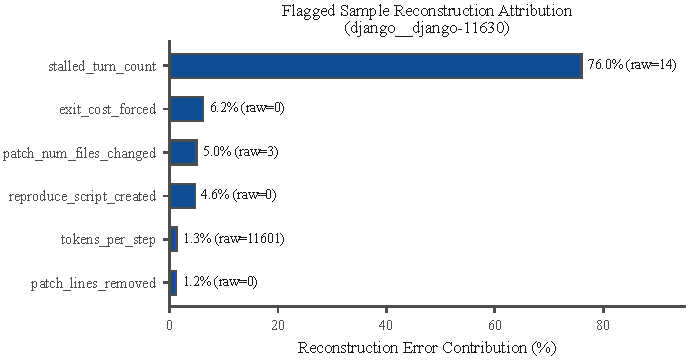
\includegraphics[width=0.72\columnwidth]{figures/fig6_feature_attribution.pdf}
\vspace{-2mm}
\caption{Per-feature reconstruction error decomposition for flagged ghostwork instance \texttt{django-11630}.}
\label{fig:interpretability}
\vspace{-2mm}
\end{figure}

\paragraph{Interpretability Attribution.}
Figure~\ref{fig:interpretability} decomposes the reconstruction error for flagged instance \texttt{django-11630} ($s(x)=112.80$). \texttt{stalled\_turn\_count} accounts for $75.98\%$ of total error (raw value 14 stalled turns), followed by \texttt{exit\_cost\_forced} ($6.19\%$). An operations engineer inspecting this attribution can immediately trust that the agent experienced command thrashing rather than constructive editing.

\paragraph{Practical Impact Translation.}
For an engineering organization executing 500 monthly agent tasks (Table~\ref{tab:practical_impact}):
Tier~2 catches 380 out of 400 failures ($95.2\%$ catch rate), reducing silent bug escapes from 60 to 20 ($-70\%$ vs. Tier~1) and false audit alerts from 30 to 8 ($-72\%$). At $\$1,200$ per production bug hotfix and $\$30$ per audit review, Tier~2 delivers a net monthly saving of \textbf{+\$48,600} over the naive heuristic.

\begin{table}[t]
\centering
\small
\resizebox{\columnwidth}{!}{
\begin{tabular}{lccc}
\toprule
\textbf{Metric (500 Tasks/Mo)} & \textbf{Tier 1 (Naive)} & \textbf{Tier 2 (Ours)} & \textbf{Tier 3 (Sup.)} \\
\midrule
Caught Failures (/400) & 340 & \textbf{380} & 337 \\
Silent Bug Escapes (FN) & 60 & \textbf{20 (-70\%)} & 63 \\
False Audit Reviews (FP) & 30 & \textbf{8 (-72\%)} & 16 \\
Net Monthly Savings & \$407,100 & \textbf{\$455,760} & \$403,920 \\
\bottomrule
\end{tabular}
}
\caption{Practical operational impact translation.}
\label{tab:practical_impact}
\end{table}

\section{Conclusion \& Limitations}\label{sec:conclusion}
\paragraph{Key Findings.}
Answering our core research question: workflow trajectory dynamics capture essential failure signals invisible in final git diffs alone, enabling a normal-only Autoencoder to achieve $0.976$ PR-AUC and $0.952$ $F_2$, matching supervised references ($p=0.565$).

\paragraph{Reflection \& Future Work.}
The most pivotal design decision was calibrating $\tau$ via validation $F_2$, which suppressed false negatives by $70\%$. To resolve the premature exit failure pattern found in Case \#3, future iterations should incorporate prompt-task semantic alignment embeddings alongside trajectory dynamics.

\paragraph{Limitations \& Deployment Considerations.}
Our study is evaluated on SWE-agent GPT-4 trajectories; cross-model distribution shifts may require periodic $\tau$ recalibration. With inference latency of $0.004$~ms, the detector introduces negligible overhead into CI/CD pipelines.

\section*{Contributions of Each Member}
\begin{itemize}
    \item \textbf{Dun-Jie Yang (Fergus4506):} Data ingestion pipeline, feature extraction, and exploratory analysis; wrote \S3--\S4.
    \item \textbf{Charlie Wang (calculusfkyou):} Tier 2 Autoencoder architecture, threshold calibration, and controlled ablations; wrote \S5 and \S7.
    \item \textbf{Mo-Ty Wang (MO7YW4NG):} Tier 1/3 baselines, 5-seed benchmark, significance tests, and error analysis; wrote \S6, \S7, and \S8.
    \item \textbf{Wei-Chia Huang (lasvigas0701):} Presentation deck design, failure case studies, conclusions, and proofreading; wrote \S1 and \S9.
\end{itemize}

\paragraph{AI Usage Statement.}
We used Claude and Gemini to assist with exploratory plotting code and polishing LaTeX formatting. All architectural decisions, experimental executions, and interpretations were conducted and verified by the authors.

\bibliography{custom}

\end{document}
